\documentclass[a4paper]{article}

\usepackage[utf8]{inputenc}
\usepackage[portuges]{babel}
\usepackage{indentfirst}
\usepackage{graphicx}
\usepackage{float}
\usepackage{caption}
\usepackage{subcaption}
\usepackage[T1]{fontenc}
\usepackage{listings}
\usepackage{amsmath}
\usepackage{mathtools}
\renewcommand{\familydefault}{\sfdefault}


\title{MEIO}
\author{MieiMasters}
\date{\today}

\begin{document}

\maketitle

\newpage

\tableofcontents


\newpage

\section{Introdução}
\label{sec:intro}

Este trabalho tem como objetivo a concepção de um modelo de simulação do funcionamento de um sistema de gestão pretendido pela empresa \textbf{ProLab} e a realização de uma simulação para o funcionamento do sistema utilizando valores alternativos para os parâmetros \textbf{S} e \textbf{s}.

Posto isto iremos então apresentar, neste relatório, todas as ideias, métodos e algoritmos que o grupo utilizou para resolver o problema proposto.

\section{Descrição e Formulação do Problema}
\label{sec:descricao}

Foi-nos apresentada uma política de gestão de inventários do tipo \textbf{Ciclo de Encomenda}. Isto significa que os pedidos de encomenda serão realizados periodicamente ao fim de cada ciclo de \textbf{t} unidades de tempo, sendo que a quantidade a ser encomendada irá variar em função do nível máximo de encomenda estabelecido (\textbf{S}) e o "\textit{stock} em mão".

No caso da política adoptada pela empresa \textbf{ProLab} existe uma pequena diferença relativamente às políticas do tipo \textbf{Ciclo de Encomenda}. A política do tipo (s,S) implica que, no final de cada ciclo \textbf{t}, a encomenda apenas é efetuada caso o \textit{stock} em mão seja inferior ao limite estabelecido \textbf{s}. Assim, só serão realizadas encomendas quando, de facto, seja imprescindível o abastecimento de \textit{stock}.

\section{Modelo de Simulação}
\label{sec:modelo}

Nesta secção iremos apresentar todo o processo de realização do modelo de simulação e, para isto, dividimo-la em três subsecções sendo estas: \textbf{Construção}, \textbf{Implementação} e \textbf{Execução}.

\begin{enumerate}
	\item Na seccção de \textbf{Construção} será apresentado todo o processo da extração de dados através da interpretação do problema apresentado.
	\item Na seccção de \textbf{Implementação} iremos atribuir significado aos dados, ou seja, explicar a utilização deles para o contexto do problema através das fórmulas para o cálculo das variáveis relevantes para o problema.
	\item Na seccção de \textbf{Execução} iremos obter os valores das variáveis pretendidas e apresentá-los.
\end{enumerate}

\newpage

\subsection{Construção}

Através dos dados que nos foram disponibilizados para a criação do modelo de simulação, o grupo construi assim a base para a obtenção dos valores analiticamente interessantes para a avaliar a eficácia e a eficiência da política de gestão a implementar.

Em primeiro lugar, retiramos a informação relativa à procura (média e devio padrão) e, de seguida, os valores possíveis para o prazo de entrega bem como as suas probabilidades respetivas.

\begin{figure}[H]
\centering
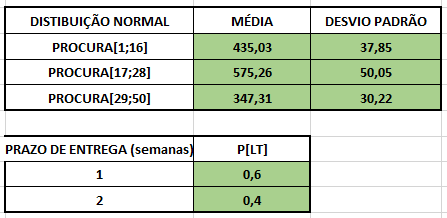
\includegraphics[scale=0.6]{distribuicaoeprazo.png}
\caption{Valores da procura e prazo de entrega}
\label{img:ProcuraePrazo}
\end{figure}

Posteriormente foram retirados os valores referentes ao juro de existência (\textbf{i}) e ao valor unitário do artigo (\textbf{b}). Através destes valores calculamos automaticamente o valor do custo de posse (\textbf{C1}).

\begin{figure}[H]
\centering
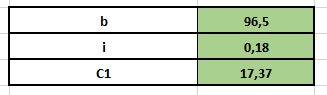
\includegraphics[scale=0.6]{Posse.png}
\caption{Custo de Posse}
\label{img:Posse}
\end{figure}

Logo após, calculamos o valor do custo de quebra (\textbf{C2}) através da fórmula: $$20+2*d1$$ sendo \textbf{d1} o último dígito do maior número mecanográfico de entre os elementos do grupo.
O custo de encomenda (\textbf{C3}) foi automaticamente retirado do enunciado tal como o ciclo de encomenda (\textbf{t}).

\begin{figure}[H]
\centering
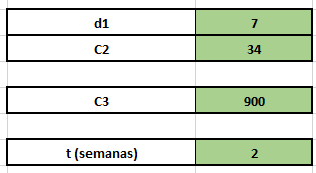
\includegraphics[scale=0.6]{c3c2t.png}
\caption{Custo de encomenda, Custo de quebra e Ciclo de encomenda}
\label{img:C3C2t}
\end{figure}

\subsection{Implementação}

\subsection{Execução}

\section{Análise Estatística dos Resultados}

\section{Resultados e Conclusões}
\label{sec:conclusao}

\end{document}
